\chapter{Risultati}%Caratterizzazione DDS su HPC
% Visti i diversi risultati si può dire che è meglio usare i topic per* le partizioni per *
% etc etc

Nella sezione corrente, vengono riportati tutti i risultati rilevanti ottenuti durante la fase di testing stilando, dove possibile, un modello di utilizzo utile alle finalità di Power Management in sistemi HPC.
\section{Discovery: centralizzata vs distribuita}
Come previsto, nella fase di discovery un numero elevato di entità genera una quantità di di pacchetti scambiati che cresce in modo esponenziale. In questo caso sono stati usati tutti i core di due nodi, con un totale di 96 entità.
Già nel primo grafico~\ref{fig:test0pack}, con il numero di pacchetti sull'asse Y e il numero di entita sull'asse X, è possibile notare una netta differenza a sole 40 unità. Nella figura~\ref{fig:test0cicl} con i cicli sulle Y, numero entità sulle X, e nella figura~\ref{fig:test0_instr} con istruzioni sulle Y, viene confermato l'andamento non lineare dell'approccio distribuito.
%TODO change 90s graph
\begin{figure}[H]
    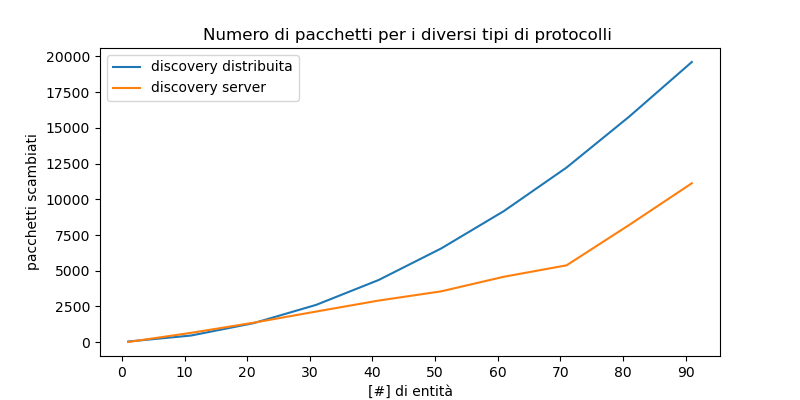
\includegraphics[width=\textwidth]{./results/test0_packet.png} 
    \caption{Numero di pacchetti scambiati durante la discovery all'aumentare di entità}\label{fig:test0pack}
\end{figure}
\begin{figure}[H]
    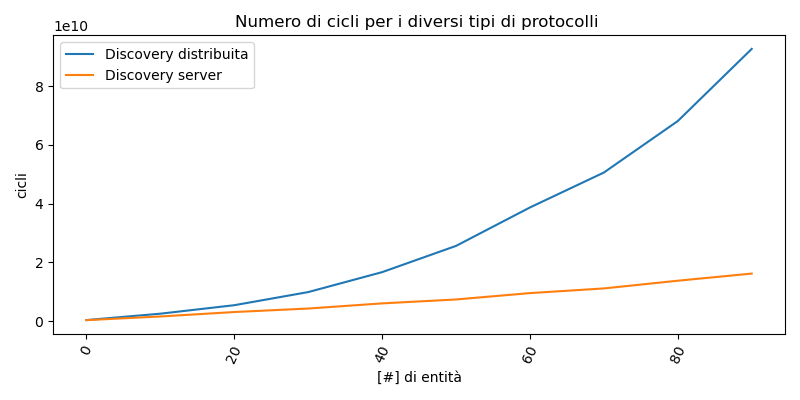
\includegraphics[width=\textwidth]{./results/test0_cicli.png} 
    \caption{Numero di cicli durante la discovery all'aumentare di entità nelle diverse opzioni}\label{fig:test0cicl}
\end{figure}
\begin{figure}[H]
    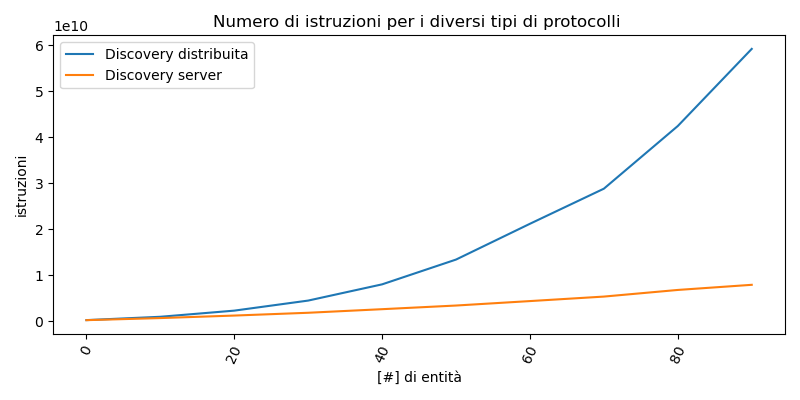
\includegraphics[width=\textwidth]{./results/test0_istruzioni.png} 
    \caption{Numero di cicli durante la discovery all'aumentare di entità nelle diverse opzioni}\label{fig:test0_instr}
\end{figure}
In un caso reale serve valutare in primo luogo il numero di entità in un determinato dominio, e successivamente i costi-benefici di ogni implementazione considerando anche l'impatto che si può avere nel caso di fallimento del server (nonostante sia possibile avere un server di backup che viene automaticamente attivato, nel caso il primo fallisse).

\section{Scalabilità del numero di entità iscritte ad un topic}
Visto lo schema~\ref{fig:uml} si può capire, che il numero di subscriber presenti in un dominio ed iscritti ad un topic, comporta un overhead di comunicazione che va ad influenzare sia i tempi, che cicli e istruzioni impiegate nella singola \emph{publish}. Questo viene dimostrato nella figura~\ref{fig:test3_overhead} (con i tempi medi di invio sulle Y) e~\ref{fig:test3_latenza} (con latenza media di ricezione in asse Y). In tutte le figure sull'asse X viene riportato il numero di subscriber che cresce fino a 40 entità. L'effetto visto è particolarmente pronunciato anche in protocolli come \emph{UDP} che non possiedono concetti di connessione. Questo potrebbe essere dovuto al costo di inizializzazione ed invio dei messaggi, ad indirizzi di rete diversi.
\begin{figure}[H]
    \centering
    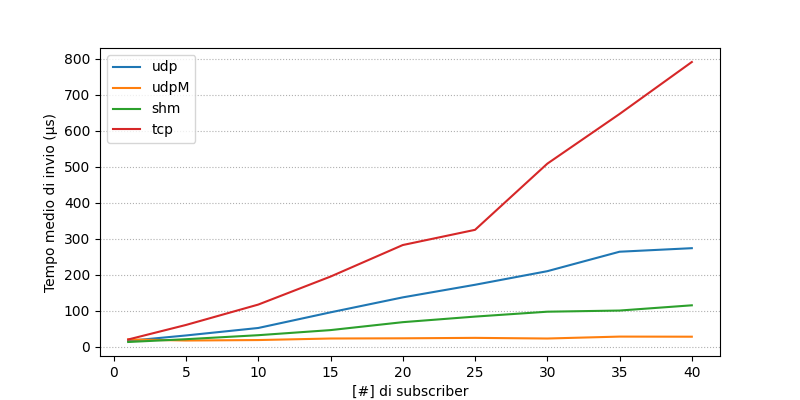
\includegraphics[width=\textwidth]{./results/test3_sending_multiplesub.png}
    \caption{Overhead sulla publish all'aumentare dei subscriber}\label{fig:test3_overhead}
\end{figure}
\begin{figure}[H]
    \centering
    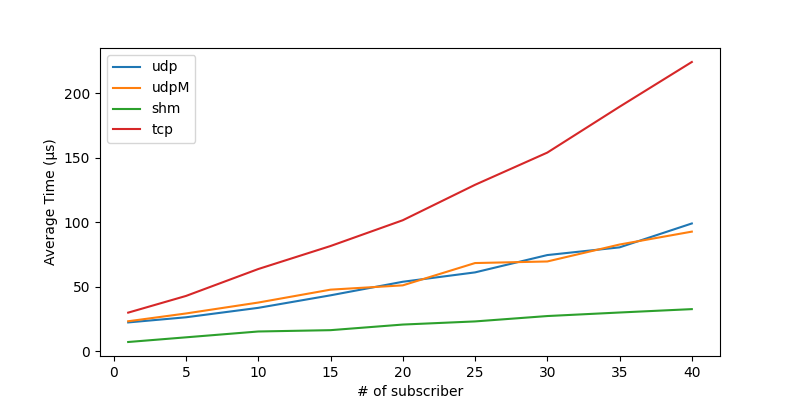
\includegraphics[width=\textwidth]{./results/test3_sendingreceiving_multiplesub.png} 
    \caption{Latenza di ricezione all'aumentare dei subscriber}\label{fig:test3_latenza}
\end{figure}

% Ovviamente l'impatto è poco significativo in quei protocolli che applicano strutture di multicasting come udp-Multicast e Shared-Memory, che verranno 

\begin{figure}[H]
        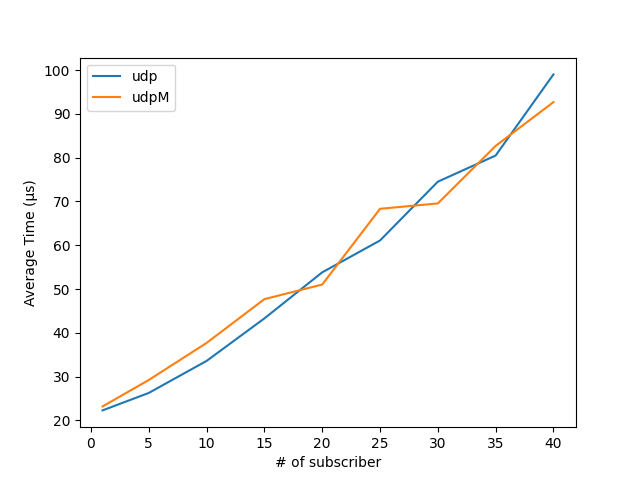
\includegraphics[width=\textwidth]{./results/test3_udpvsudpM.png} 
        \caption{Tempo di invio di un messaggio a [\#] subscriber nei protocolli UDP e UDP Multicast}\label{fig:udpvsudpMfigure}
\end{figure}

Da questo si può concludere che sia il publisher che subscriber risente della presenza di molteplici \emph{dds-partecipant} in ascolto su un topic. Questo problema è migliorato nel caso vengano utilizzati protocolli che si basano su multicast. Nel caso vengano richieste velocità elevate di comunicazione è quindi preferibile utilizzare domini e partizioni di comunicazione non eccessivamente grandi.

\section{Overhead sul primo messaggio}
E' stato notato con tutti i protocolli utilizzati un ritardo, di un ordine di grandezza superiore, che riguarda esclusivamente il primo messaggio. Tuttavia, non è stato chiarito il motivo di questo overhead, presente anche in comunicazioni locali\footnote{comunicazioni effettuati in localhost o in shared memory}. Anche se non dimostrato una delle possibili motivazioni potrebbe essere la necessità di allocare memoria durante la prima fase di comunicazione~(\ref{sec:rtps}), da entrambi gli attori (potenzialmente amplificato nel caso~\ref{fig:rtt_uml}). In figura~\ref{fig:overhead_primo_messaggio} con tempo di ricezione sull'asse Y e sequenza dei messaggi sull'asse X, viene mostrato il problema citato.
\begin{figure}[H]
    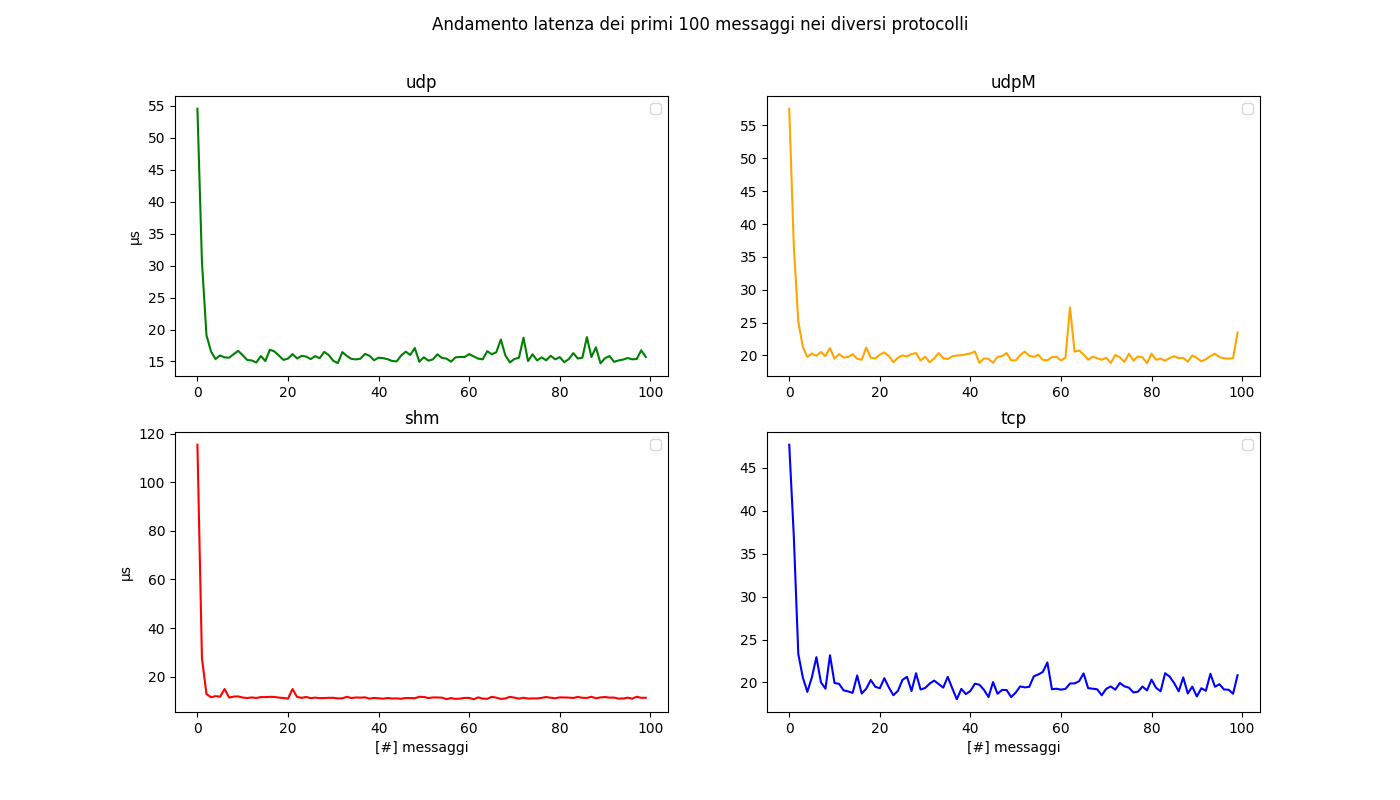
\includegraphics[width=\textwidth]{./results/errortest.png} 
    \caption{Overhead del primo messaggio nei vari protocolli}
    \label{fig:overhead_primo_messaggio}
\end{figure}
Infine, vista la mancanza di approfondimento verso tale problema, non si può concludere che l'invio di pochi messaggi sia sfavorito in questa implementazione.

\section{Protocolli di comunicazione}
Visti gli schemi~\ref{fig:minpowerstackscheme} è risulta probabile che in un Power Stack, siano predilette le comunicazioni non locali. In merito a ciò, nonostante ci siano di mezzo molti più livelli per comunicare con udp e tcp, i risultati trovati sono stati decisamente interessanti e non così lontani dal più veloce \emph{Shared Memory}. 
In figura~\ref{fig:test3_different_protocols} sugli assi X il numero di subscriber, e sulle Y le latenza di ricezione in microsecondi, vengono mostrati i risultati separati per tutti i protocolli.
\begin{figure}[H]
    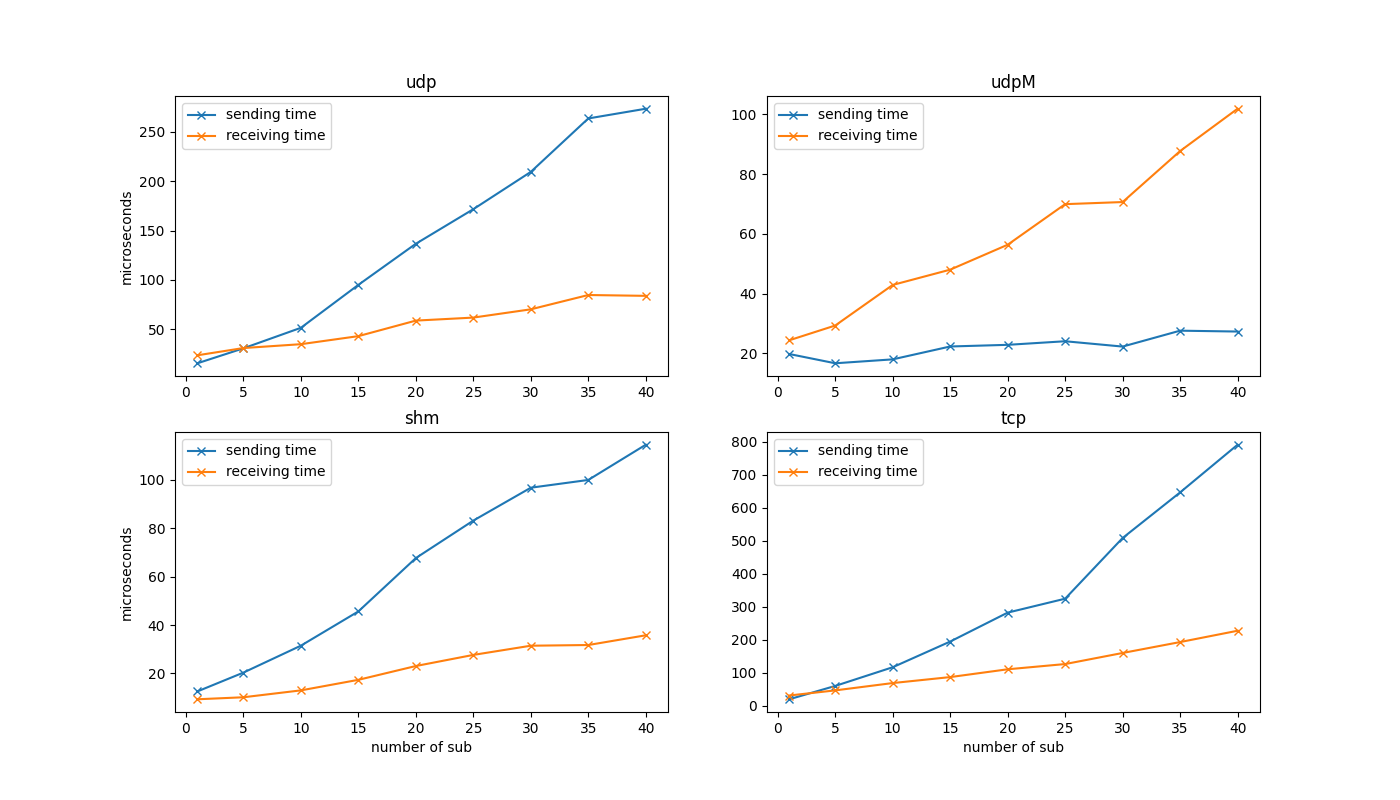
\includegraphics[width=\textwidth]{./results/test3_different_protocol_send_receive.png} 
        \caption{Differenza della latenza di ricezione dei vari protocolli con }\label{fig:test3_different_protocols}
\end{figure}
In figura~\ref{fig:test3_different_protocols2} sugli assi X i protocolli, mentre sulle Y le latenza di ricezione in microsecondi vengono confrontati i valori per un singolo messaggio, mentre e figura~\ref{fig:test1sdbox} le variazioni di questi risultati.

\begin{figure}[H]
    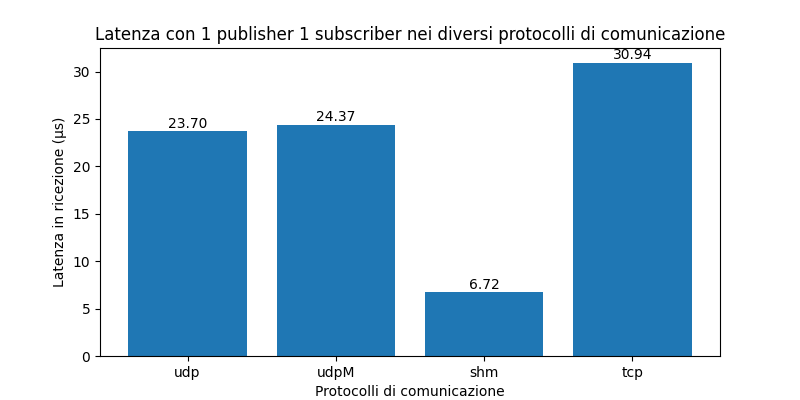
\includegraphics[width=\textwidth]{./results/test1_bar_sr_1p1s.png} 
        \caption{Latenza media di ricezione di un singolo messaggio nei vari protocolli}\label{fig:test3_different_protocols2}
\end{figure}

\begin{figure}[H]
    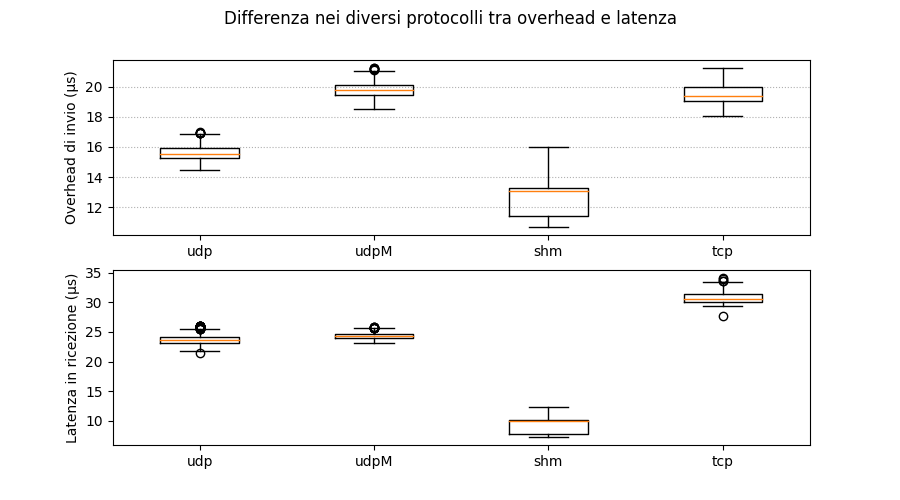
\includegraphics[width=\textwidth]{./results/test1_box_sr_1p1s.png} 
        \caption{Diagramma a scatola nei vari protocolli di comunicazione con un publisher e un subscriber}\label{fig:test1sdbox}
\end{figure}
Infine, in figura~\ref{fig:test3_cycle_different_protocols} con protocolli sull'asse X e conteggio di cicli e istruzioni ($10^6$) su Y, viene mostrato l'overhead computazionale di ognuno dei meccanismi proposti.
\begin{figure}[H]
    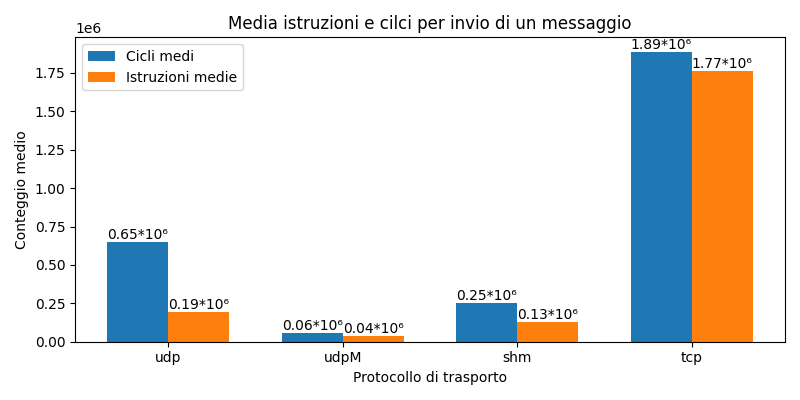
\includegraphics[width=\textwidth]{./results/test1_cyclinstr.png} 
        \caption{Conteggio cicli e istruzioni per ogni protocollo}\label{fig:test3_cycle_different_protocols}
\end{figure}
E' quindi preferibile, ove possibile, usare \emph{Shared Memory} sia per prestazioni, che per evitare di saturare la rete. In secondo luogo, se in presenza di diversi subscriber, per non caricare il publisher usare \emph{UDP Multicast}. E infine utilizzare \emph{TCP} solo dove vi è necessità di connessione, visto le notevoli latenze si in scrittura che in lettura. In tutti gli altri casi, dove non si è in locale, e dove il numero di subscriber non supera qualche decina, risulta più che adeguato \emph{UDP}.

\section{Domini, Partizioni e Wildcards}
Nei test effettuati con topic e partizioni, non sono state notate differenze degne di nota in termini di performance nell'usare uno strumento piuttosto che un altro (\ref{fig:test2parttopicdomain}). Lo sono stati invece tra questi ultimi e i Domini. Tuttavia i domini non offrono alcun tipo di flessibilità e richiede il riavvio dei \emph{dds-partecipant} nel caso si necessiti di un qualsiasi cambiamento. Per questo è consigliato utilizzo di domini diversi, solo tra entità che non hanno necessità di comunicare, e che anzi, magari anche per motivi di sicurezza devono stare isolati. 
In figura~\ref{fig:test2parttopicdomain} sugli assi X il numero crescente di subscriber, e sulle Y conteggio medio di cicli ($10^6$).

\begin{figure}[H]
    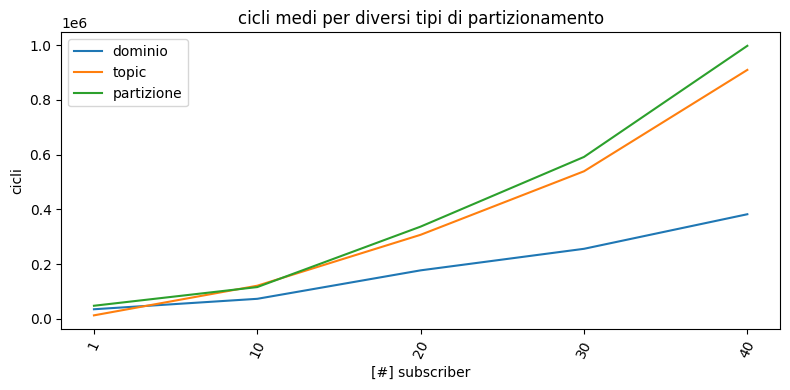
\includegraphics[width=\textwidth]{./results/test2_cicli_partvstopicvsdomaain.png} 
        \caption{Peso in termini di cicli nell'usare partizioni topic e domini}\label{fig:test2parttopicdomain}
\end{figure}

Per quanto riguarda entità che necessitano di gerarchie, è conveniente usare le partizioni con le Wildcards visto che non hanno un peso significativo come notabile in~\ref{fig:test2wildcards} dove sull'asse X vi è il numero di partizioni usate, mentre sulle Y il tempo di invio. Infine lasciando i topic come mezzo di partizionamento predefinito, per il tipo di dati, e il tipo di istruzioni da utilizzare.

\begin{figure}[H]
    \centering
    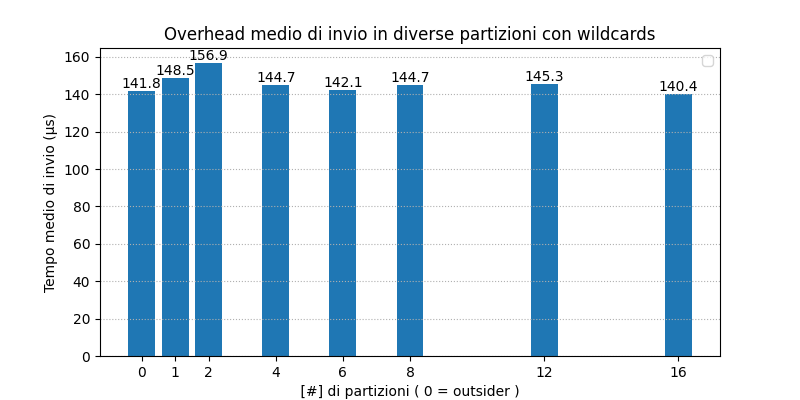
\includegraphics[width=\textwidth]{./results/test2_wildcards.png}

    \caption{Differenza in tempi di invio con utilizzo di wildcards in diverse partizioni}\label{fig:test2wildcards}
\end{figure}
Questo viene confermato anche nella figura \ref{fig:test2cicl}, dove viene mostrato l'overhead computazionale sull'asse Y tramite conteggio di istruzioni e cicli ($10^6$), rispetto al numero gruppi presenti (sulla X), utilizzando le wildcards.
\begin{figure}[H]
    \centering
    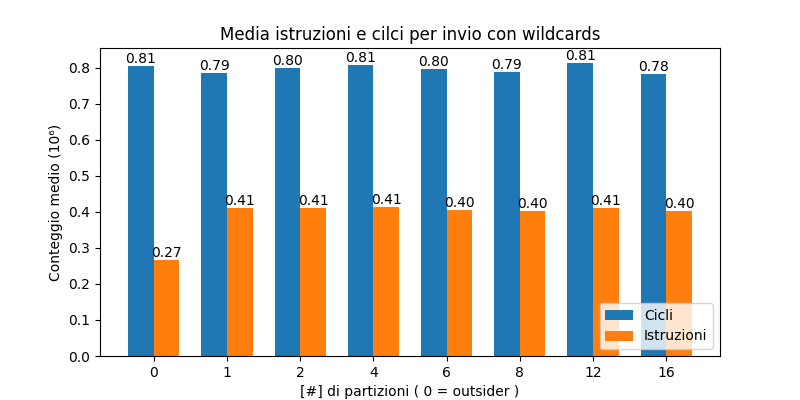
\includegraphics[width=\textwidth]{./results/test2_cyclinstr.png}
    \caption{Cicli e istruzioni necessari per invio con wildcards in diverse partizioni}\label{fig:test2cicl}
\end{figure}




\section{Throughput} % da sistemare test3 bandwidth, throughput e Freqeuncy
L'ultimo test, rivolto alla caratterizzazione della capacità di comunicazione, del middleware DDS, ci permette di capire il massimo scambio di dati che può avvenire tra i vari attori del Power Management. Nella figura \ref{fig:throughput_combined} l'asse Y, a sinistra, mostra in verde i il valore di KMessaggi/s~\footnote{1000 Messaggi al secondo} raggiungibili dai vari protocolli di comunicazione (in asse X), mentre in grigio, a destra i KByte/s. Dalla figura si può vedere che è possibile inviare ogni secondo da un publisher ad un subscriber più di un MB/s di dati. Inoltre è possibile raggiungere frequenze di scambio di messaggi dell'ordine di decine di KHz (\ref{fig:throughput_combined}). Inoltre, nel caso di invii a più subscriber, come si può vedere in figura~\ref{fig:bandwidth_graph}, mentre i protocolli udp shm tcp saturano all'aumentare del numero di subscriber, il protocollo UDP Multicast, permette una crescita lineare del throughput.

\begin{figure}[H]
    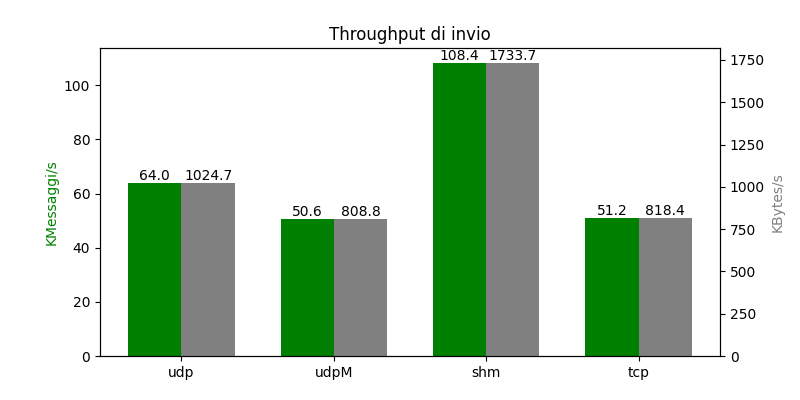
\includegraphics[width=\textwidth]{./results/test3_throughput_combined.png} 
        \caption{Throughput con un publisher e un subscriber}\label{fig:throughput_combined}
\end{figure}

\begin{figure}[H]
    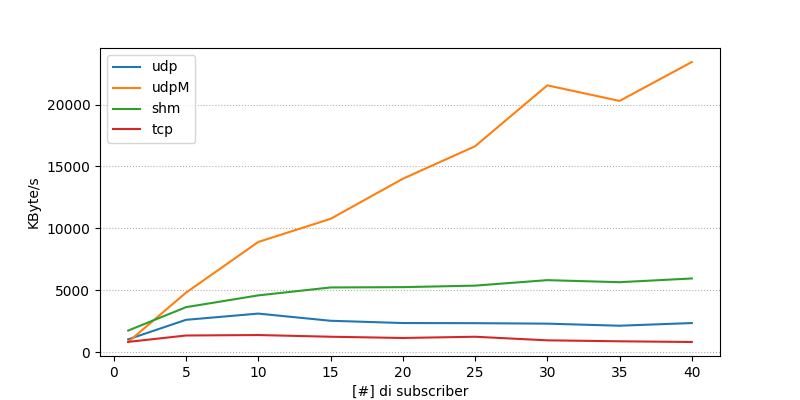
\includegraphics[width=\textwidth]{./results/test3_graph_throughput.png} 
    \caption{Throughput a crescenti numeri di subscribers}\label{fig:throughput_increasing}
\end{figure}

Il risultato ottenuto nelle figure \ref{fig:throughput_combined} \ref{fig:throughput_increasing} (KBytes/s sulla Y e numero di subscriber sulla X), per quanto riguarda il protocollo UDP Multicast, è influenzato dalla struttura del test mostrato in figura \ref{fig:rtt_uml}, che non permette ad UDP Multicast di mostrare le sue potenzialita, come invece si può vedere dalla figura \ref{fig:bandwidth_graph}.

\begin{figure}[H]
    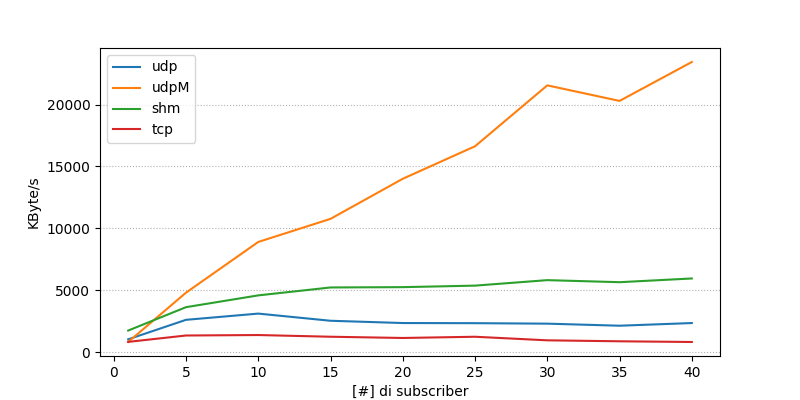
\includegraphics[width=\textwidth]{./results/test3_graph_bandwidth.png} 
        \caption{capacità di invio in KByte/s da un publisher a molteplici subscriber}\label{fig:bandwidth_graph}
\end{figure}

% Nella figura \ref{fig:bandwidth_combined} viene mostrato come un publisher usando multicast, viene liberato del suo incarico di inviare il messaggio ad ogni indirizzo di ogni subscriber, inviandolo ad un semplice indirizzo dove tutti i publisher riescono a 

